\documentclass[12pt,titlepage]{article}
\usepackage[dvipsnames,rgb,dvips,table]{xcolor}
\usepackage{graphicx,caption}
\graphicspath{../Figures/}
\usepackage{psfrag}
\usepackage{dcolumn}
\usepackage{bm}
\usepackage{amsmath}
\usepackage{amssymb}
\usepackage[rflt]{floatflt}
\usepackage{latexsym}
%\usepackage{float}
\usepackage{bm}
\usepackage{subcaption}
\usepackage{booktabs}
\usepackage{floatrow}
\floatsetup[table]{font=footnotesize}
\usepackage[hidelinks]{hyperref}
\usepackage{array}
\usepackage{ragged2e}
\newcolumntype{P}[1]{>{\RaggedRight\hspace{0pt}}p{#1}}
\usepackage{color}
\usepackage[bottom]{footmisc}

\usepackage[left=20mm,right=20mm,top=25mm,bottom=20mm]{geometry}


\pagestyle{myheadings}
\markright{{\small Jacopo Credi \hfill (910216-T396) \,}}
\DeclareMathOperator\erf{erf}
\author{Jacopo Credi \\(910216-T396) \\ \vspace*{2cm} }
\title{{\Large \textsc{Chalmers University of Technology}} \\ \bigskip FFR135 - Artificial Neural Networks\\ \bigskip Examples sheet 3 \\ \vspace*{2cm}}

\usepackage{listings}
\usepackage{color} %red, green, blue, yellow, cyan, magenta, black, white
\definecolor{mygreen}{RGB}{28,172,0} % color values Red, Green, Blue
\definecolor{mylilas}{RGB}{170,55,241}
% Settings for writing Matlab code
\lstset{language=Matlab,%
	basicstyle=\small\ttfamily,
    %basicstyle=\color{red},
    breaklines=true,%
    morekeywords={matlab2tikz},
    keywordstyle=\color{blue},%
    morekeywords=[2]{1}, keywordstyle=[2]{\color{black}},
    identifierstyle=\color{black},%
    stringstyle=\color{mylilas},
    commentstyle=\color{mygreen},%
    showstringspaces=false,%without this there will be a symbol in the places where there is a space
    numbers=left,%
    numberstyle={\tiny \color{black}},% size of the numbers
    numbersep=9pt, % this defines how far the numbers are from the text
    %emph=[1]{for,end,break},emphstyle=[1]\color{red}, %some words to emphasise
    frame=single,                   % adds a frame around the code
  	rulecolor=\color{black},
    %emph=[2]{word1,word2}, emphstyle=[2]{style},    
}


\setlength{\parskip}{3pt}

\begin{document}
\parindent=0cm
\maketitle

\subsection*{Problem 1}

\begin{table}[H]
\resizebox{\textwidth}{!}{
\begin{tabular}{llcc}
\toprule
\textbf{Classes} & \textbf{Subclasses} & \textbf{LS} & \textbf{n$^o$ configurations} \\
\toprule
1) All of the same colour & (none) & \textcolor{blue}{yes} & \textcolor{blue}{2} \\
\midrule
2) 1 of a colour, 7 of the other & (none) & \textcolor{blue}{yes} & \textcolor{blue}{16} \\
\midrule
3) 2 of a colour, 6 of the other &
\begin{tabular}{@{}l@{}}
	3a) Two vertices sharing an edge\\
	3b) Two vertices on square diagonal\\
	3c) Two vertices on cube diagonal \\
\end{tabular} & 
\begin{tabular}{@{}l@{}}
	\textcolor{blue}{yes} \\
	\textcolor{red}{no}  \\  
	\textcolor{red}{no} \\ 
\end{tabular}  & 
\begin{tabular}{@{}l@{}} 
	\textcolor{blue}{24} \\ 
	\textcolor{red}{24}  \\ 
	\textcolor{red}{8} \\ 
\end{tabular}  \\
\midrule
4) 3 of a colour, 5 of the other &
\begin{tabular}{@{}l@{}}
	4a) Three vertices forming a V \\
	4b) Two vertices adjacent, third on opposite edge\\
	4c) Three non-adjacent vertices \\
\end{tabular} & 
\begin{tabular}{@{}l@{}}
	\textcolor{blue}{yes} \\
	\textcolor{red}{no}  \\  
	\textcolor{red}{no} \\ 
\end{tabular}  & 
\begin{tabular}{@{}l@{}} 
	\textcolor{blue}{48} \\ 
	\textcolor{red}{48}  \\ 
	\textcolor{red}{16} \\ 
\end{tabular}  \\
\midrule
5) 4 of a colour, 4 of the other &
\begin{tabular}{@{}l@{}}
	5a) Four vertices on a cube face \\
	5b) Four vertices forming a star\\
	5c) Vertices adjacent two by two, on opposite edges\\
	5d) Vertices forming two connected perpendicular V's \\
	5e) Three vertices forming a V, fourth non-adjacent \\
	5f) Four non-adjacent vertices  \\
\end{tabular} & 
\begin{tabular}{@{}l@{}}
	\textcolor{blue}{yes} \\
	\textcolor{blue}{yes} \\
	\textcolor{red}{no}  \\  
	\textcolor{red}{no} \\
	\textcolor{red}{no}  \\  
	\textcolor{red}{no} \\	
\end{tabular}  & 
\begin{tabular}{@{}l@{}} 
	\textcolor{blue}{6} \\ 
	\textcolor{blue}{8} \\
	\textcolor{red}{6}  \\ 
	\textcolor{red}{24} \\ 
	\textcolor{red}{24}  \\ 
	\textcolor{red}{2} \\ 
\end{tabular}  \\
\toprule
 & & \textcolor{blue}{Subtotal LS} & \textcolor{blue}{104} \\
 & & \textcolor{red}{Subtotal non-LS} & \textcolor{red}{152} \\
 \cmidrule{3-4}
 & & \textbf{Total} & 256 \\
\end{tabular}}
\caption{\footnotesize Classification of  Boolean functions with three inputs in (sub)classes of linearly separable (LS) and non LS functions, seen as the problem of colouring the vertices of a cube with two colours.}
\label{tab:1}
\end{table}

\subsubsection*{Discussion}
The problem of classifying three-input Boolean functions as linearly separable (LS) or not can be visualised as the problem of colouring the vertices of a $(2 \times 2 \times 2)$-cube with two colours and then finding a plane separating vertices of different colour.

Table~\ref{tab:1} describes the different classes and subclasses of colouring configurations, the number of such configurations in each subclass and whether they are linearly separable (LS) or not. The subclasses were found by visualising the $(2 \times 2 \times 2)$-cube and considering the possible ways of colouring $n$ vertices with one colour and $8-n$ with the other colour, for $n \in \lbrace0,1,2,3,4\rbrace$ (other cases are symmetrical). The number of configurations in each subclass was found by considering all possible rotations and reflections of a configuration of the subclass.

Out of the $2^{2^3} = 256$ Boolean functions with three inputs, $104$ are found to be linearly separable and $152$ non-linearly separable.
\clearpage

\newgeometry{left=20mm,right=20mm,top=22mm,bottom=17mm}
\subsection*{Problem 2(a)}

\vspace*{-0.5cm}
\begin{figure}[H]
\centering
    \begin{subfigure}[b]{0.57\textwidth}
        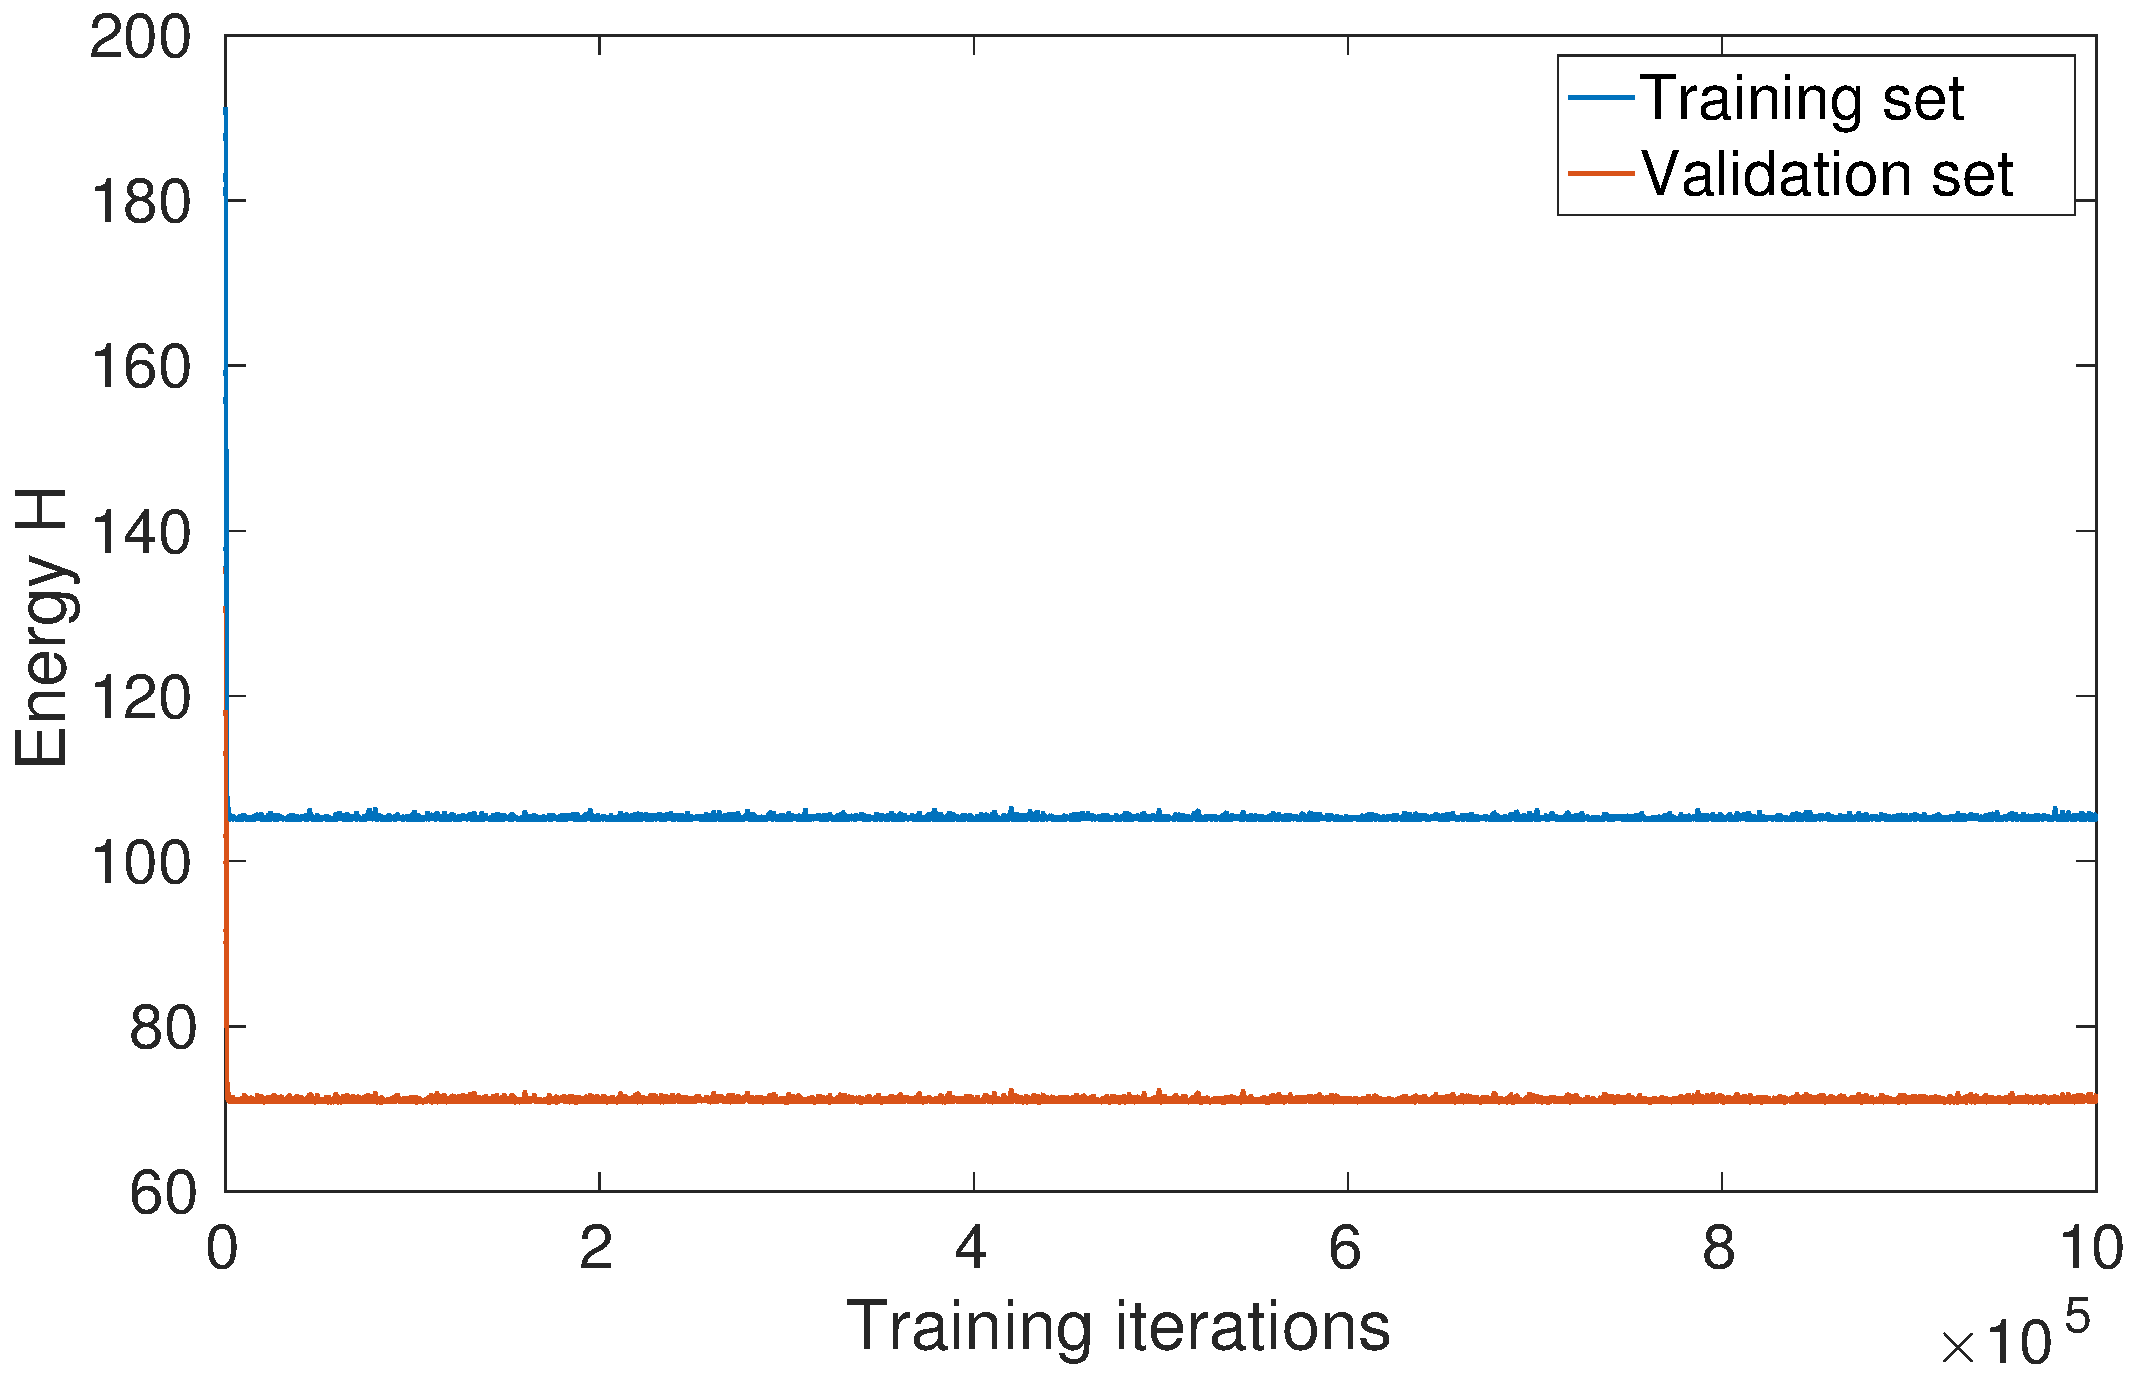
\includegraphics[width=\textwidth]{../Figures/noHL_energy.pdf}
        \caption{}
    \end{subfigure} %
    \hfill %
    \begin{subfigure}[b]{0.39\textwidth}
        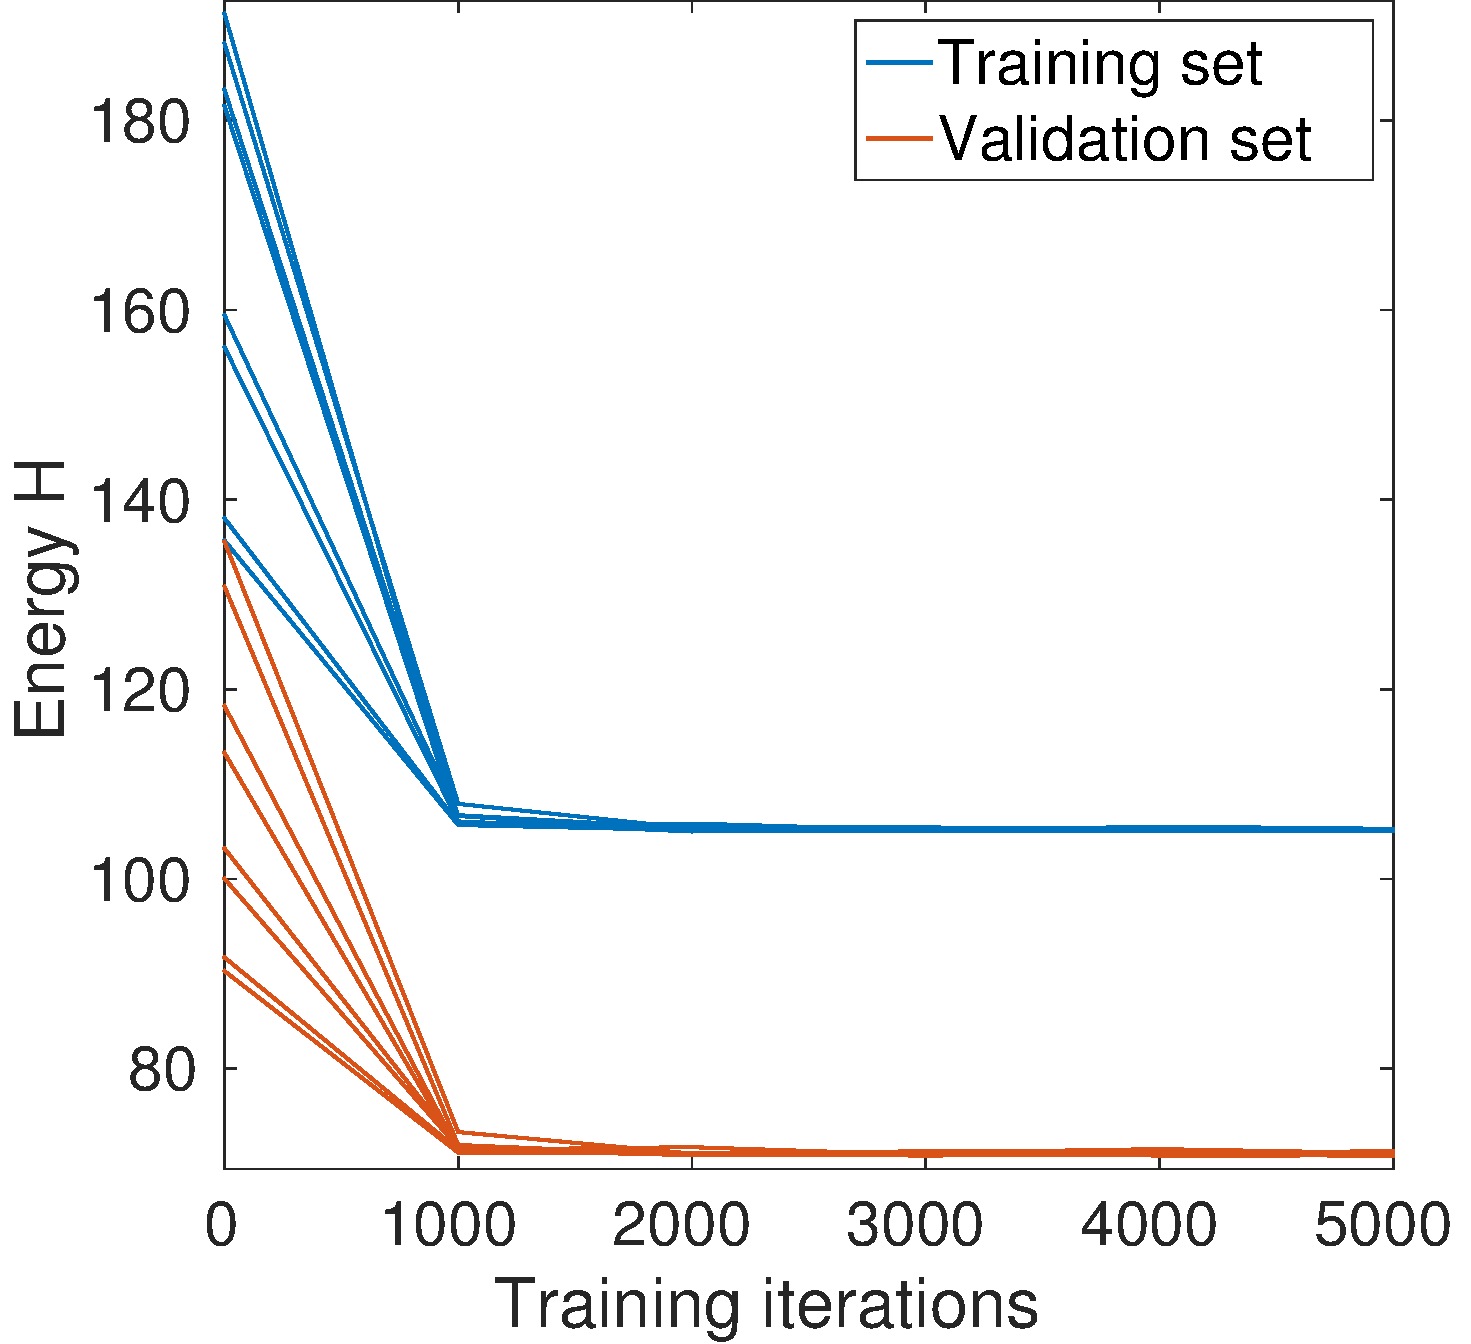
\includegraphics[width=\textwidth]{../Figures/noHL_energy_part.pdf}
        \caption{}
    \end{subfigure} %
    \vspace*{-0.2cm}
\caption{\footnotesize Left panel: energy $H$ vs training iterations for both the training set (blue) and the validation set (red). Energy was evaluated every 1000 iterations. Ten independently initialised runs are displayed, with the same colour-coding. Right panel: zoom of the first 5000 iterations.}
\label{fig:2a}
\end{figure}

\vspace*{-0.4cm}
\subsubsection*{Discussion}
\vspace*{-0.3cm}
A simple perceptron with 2 input neurons, 1 output neuron and no hidden layer was trained with asynchronous backpropagation algorithm, using the provided training data. Data was first preprocessed, by subtracting the sample mean and dividing by the sample standard deviation.

Network weights were initialised randomly with uniform distribution in $[-0.2, 0.2]$ and biases with uniform distribution in $[-1, 1]$. The activation function was taken to be $g(z) = \tanh(\beta z)$, with parameter $\beta = 1/2$. The learning rate was set to $\eta = 0.01$. Ten independently initialised training runs were performed, with $10^6$ training iterations in each run.

At each iteration, a random pattern $\bm{\xi}^{(\mu)}$ is used as input and the output value is computed using McCulloch-Pitts dynamics, i.e. $O^{(\mu)} = g(b)$, where $b = \bm{w} \ \bm{\xi}^{(\mu)}$ and the threshold/bias is incorporated in the weight vector $\bm{w}$, using an extra (dummy) neuron with fixed state $-1$. The weights are then updated as $\bm{w} \rightarrow \bm{w}+ \bm{\delta w}$, with $\bm{\delta w} = \eta \ \Delta \ (\bm{\xi}^{(\mu)})^T$, where $\Delta = (\zeta^{(\mu)} - O^{(\mu)}) g'(b)$.

As shown in Fig.~\ref{fig:2a}, energy initially drops very quickly (see panel b), but it then stabilises around 105 for the training set and 71 for the validation set. The difference in the energy value between training and validation sets can be explained by considering that the data sets have different size (energy is indeed an ``extensive'' property of the system) and therefore different values are not indicative of different performance (in fact $105/71 \simeq 1.5$, which is the ratio of the data sets size).

Since the backpropagation algorithm is based on gradient descent, the energy $H$ is expected not to increase if using batch mode. However, in asynchronous backpropagation, energy in general exhibits oscillations (and therefore can slightly increase), depending on the learning rate $\eta$. The effect $\eta$ was investigated by performing some additional training runs with ${\eta \in [0.001, 0.1]}$. As one can expect, a very small $\eta$ slows down the training, but yields smaller energy oscillations, whereas a larger $\eta$ increases the learning speed, but leads to stronger oscillations. \looseness=-1

\vspace*{-0.4cm}
\subsubsection*{Reference code}
\vspace*{-0.3cm}
See \textsc{matlab} script \verb!MultilayerPerceptronBackpropagation.m! and custom functions used in the script itself, in particular \verb!RunPerceptron.m!, \verb!Backpropagation.m! and \verb!ComputeErrorAndEnergy.m!.
\enlargethispage{\baselineskip}


\clearpage
\restoregeometry


\subsection*{Problem 2(b)}

\vspace*{-0.3cm}
\begin{figure}[H]
\centering
    \begin{subfigure}[b]{0.58\textwidth}
        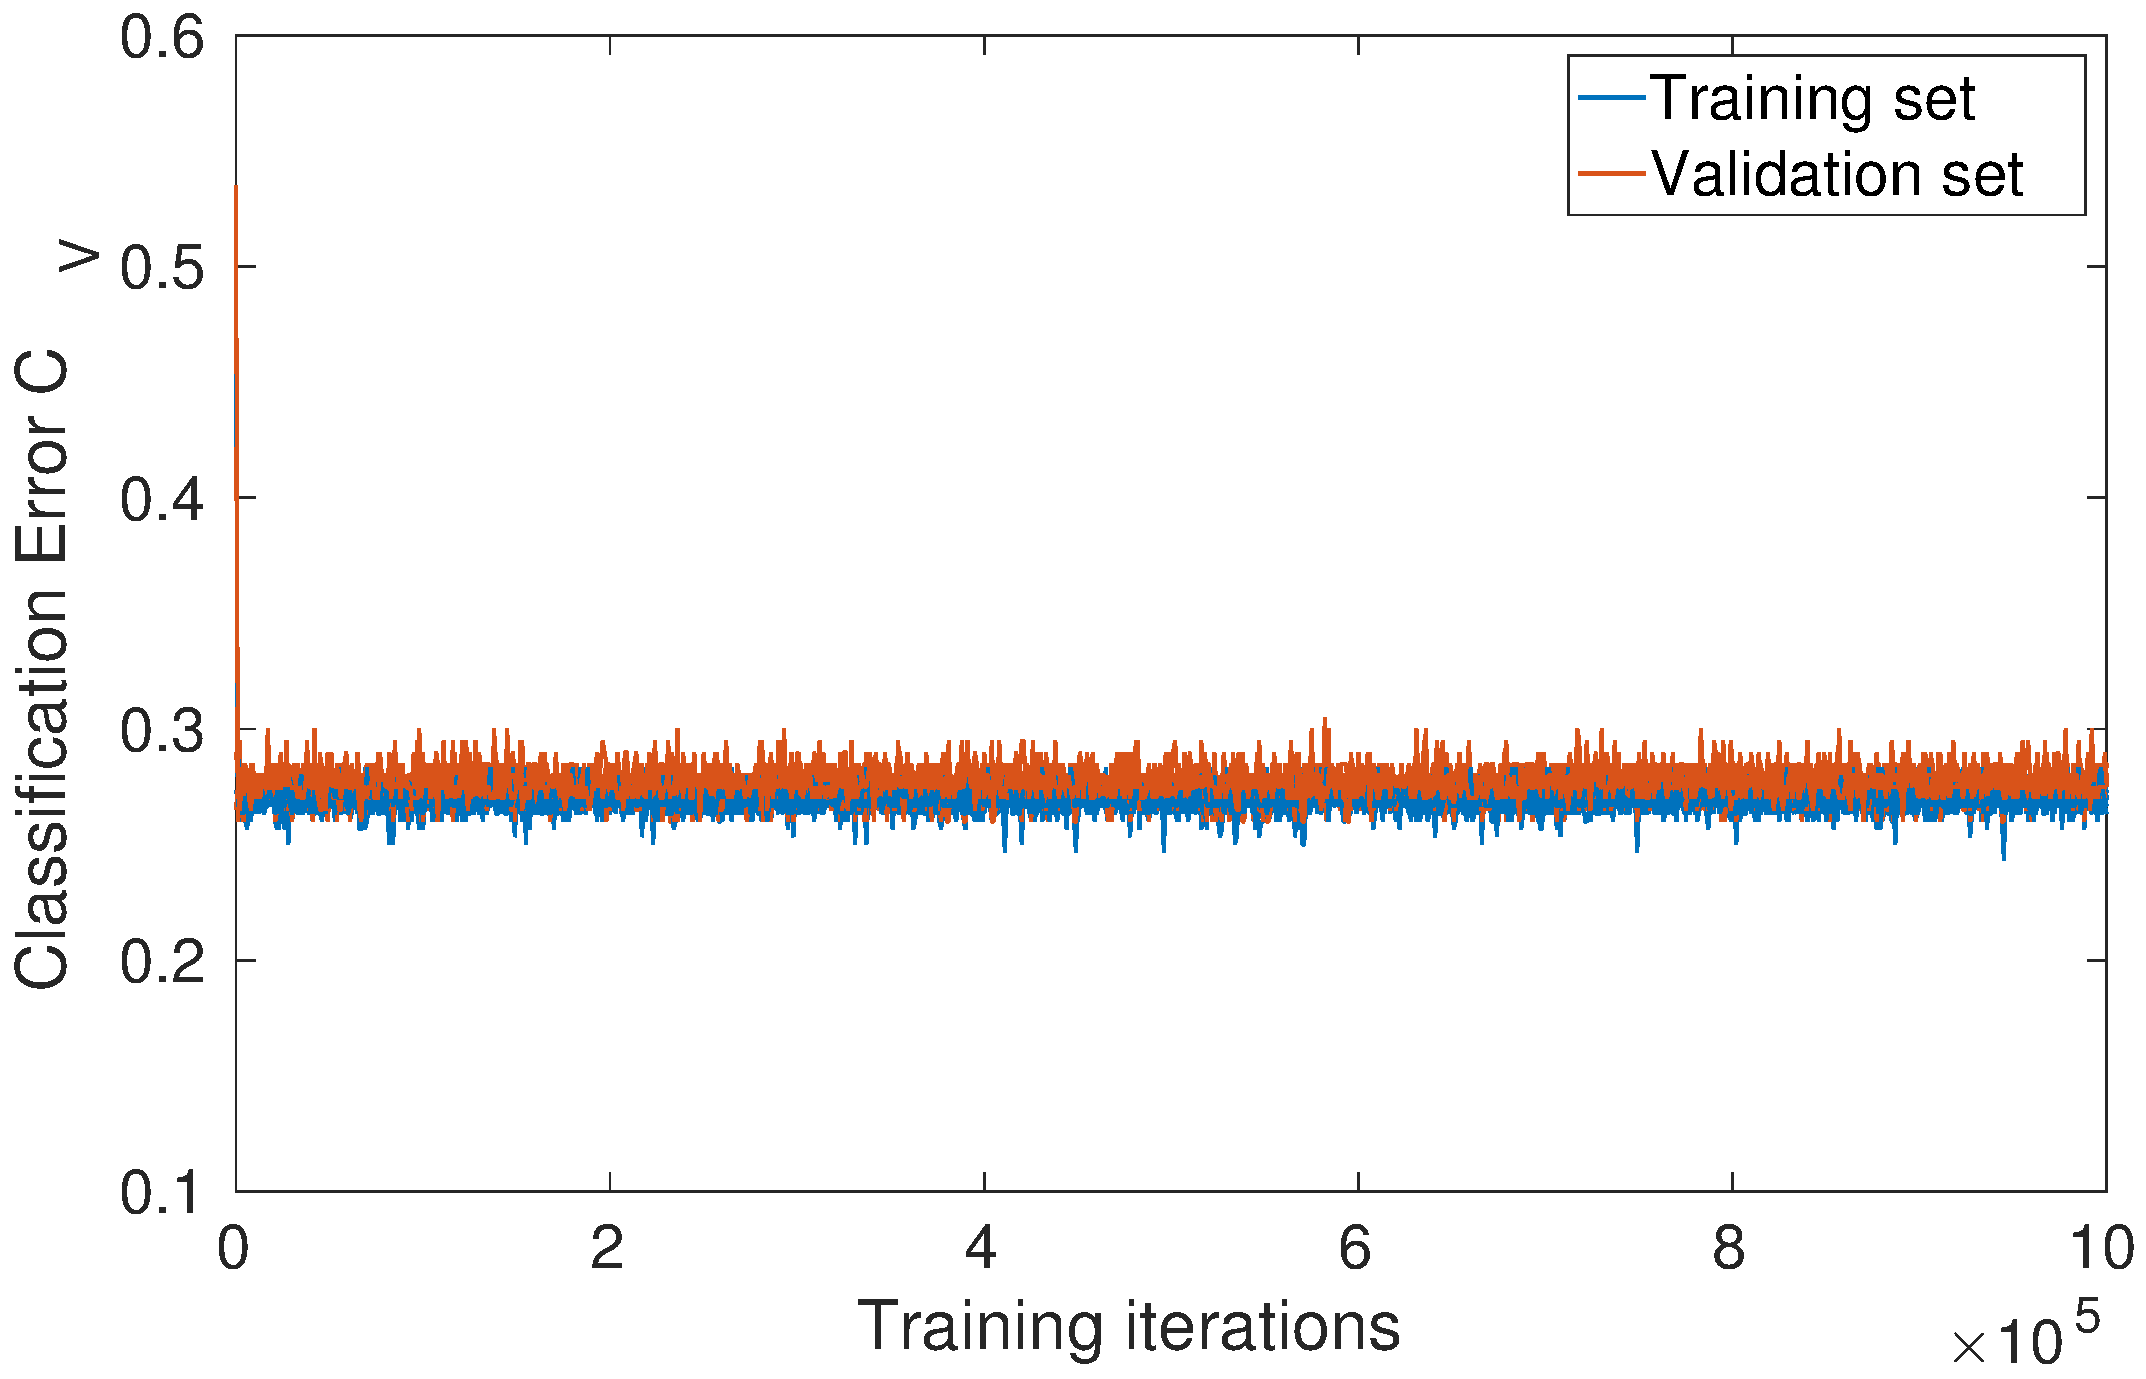
\includegraphics[width=\textwidth]{../Figures/noHL_error.pdf}
        \caption{}
    \end{subfigure} %
    \hfill %
    \begin{subfigure}[b]{0.4\textwidth}
        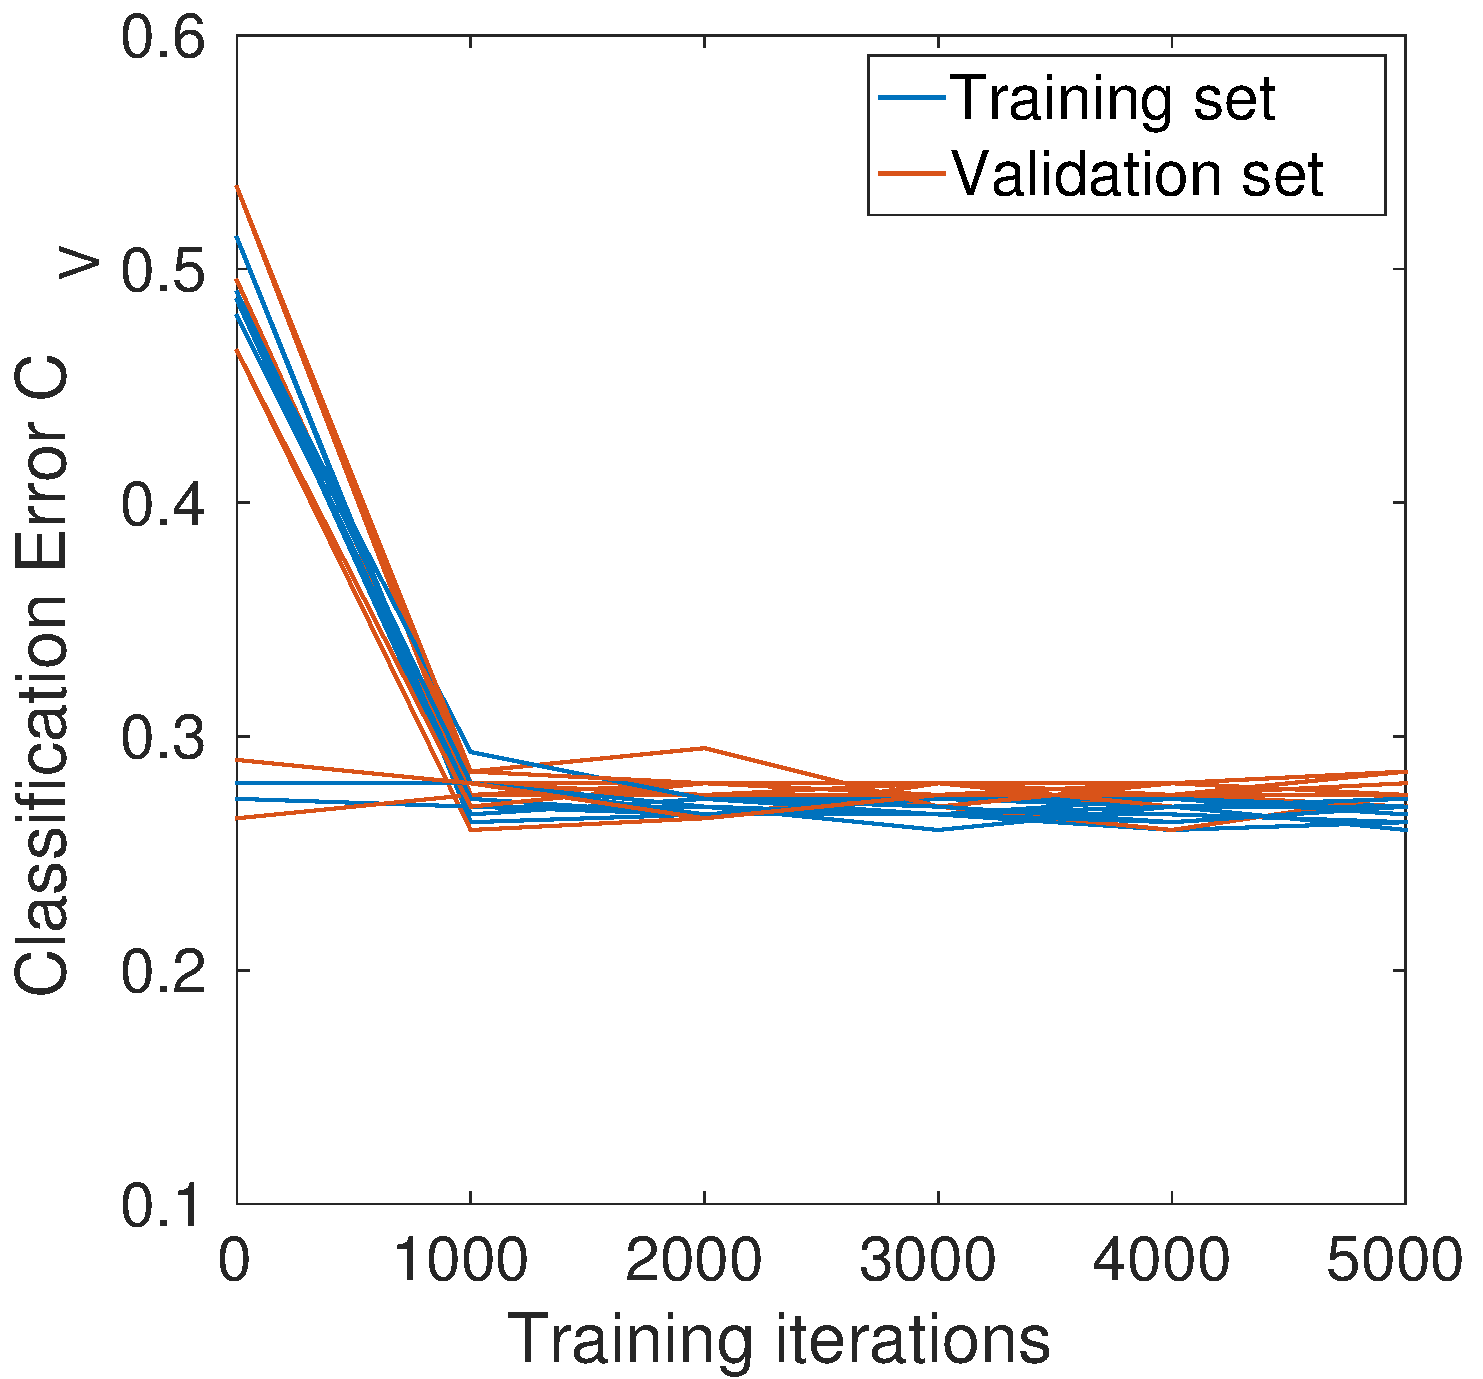
\includegraphics[width=\textwidth]{../Figures/noHL_error_focus.pdf}
        \caption{}
    \end{subfigure} %
\caption{\footnotesize Left panel: classification error $C_V$ vs training iterations for both the training set (blue) and the validation set (red). One point every 1000 iterations is shown. Ten independently initialised runs are displayed, with the same colour-coding. Right panel: zoom of the first 5000 iterations.}
\label{fig:2b}
\end{figure}

\vspace*{-0.2cm}
\subsubsection*{Discussion}
\vspace*{-0.3cm}
The classification error of a data set with one output is defined as
\vspace*{-0.1cm}
\begin{equation}
C_V = \dfrac{1}{2p} \ \sum_{\mu = 1}^p \mid \zeta^{(\mu)} - \text{sgn}(O^{(\mu)}) \mid \ , 
\end{equation}%
where $p$ is the number of patterns in the set and the factor $1/2$ was added to have $C_V \in [0,1]$.

The classification error was computed every $1000$ training iterations for both the training and the validation set (Fig.~\ref{fig:2b}). These plots clearly show that the classification performance of this simple perceptron is quite poor: even though the error quickly drops from around 0.5 (i.e. random classification) to around 0.27 for both training and validation sets, it does not really decrease any further in the rest of the training process.

In other terms, the perceptron is incorrectly classifying patterns more than $25\%$ of the time, suggesting that this simple network architecture is unsuitable for the function that we are trying to approximate. The reason for this is that such function is not linearly separable, as one can notice by a quick plot of the patterns.

In the geometric interpretation of straight lines (or, in general, hyperplanes) separating points in the input space, the above results mean that the best straight line found by the backpropagation algorithm 
is such that around $27\%$ of the points classified as ``+1'' actually lie below the line itself, and around $27\%$ of the points classified as ``-1'' actually lie above it.

The difference between errors obtained in different runs is negligible, as there are no ``local optima'' to get stuck in. All training runs are equally good, or more precisely equally bad.

\vspace*{-0.2cm}
\subsubsection*{Reference code}
\vspace*{-0.2cm}
See \textsc{matlab} script \verb!MultilayerPerceptronBackpropagation.m! and custom functions used in the script itself, in particular \verb!RunPerceptron.m!, \verb!Backpropagation.m! and \verb!ComputeErrorAndEnergy.m!.

\clearpage

\subsection*{Problem 2(c)}
\vspace*{-0.3cm}
\begin{figure}[H]
\centering
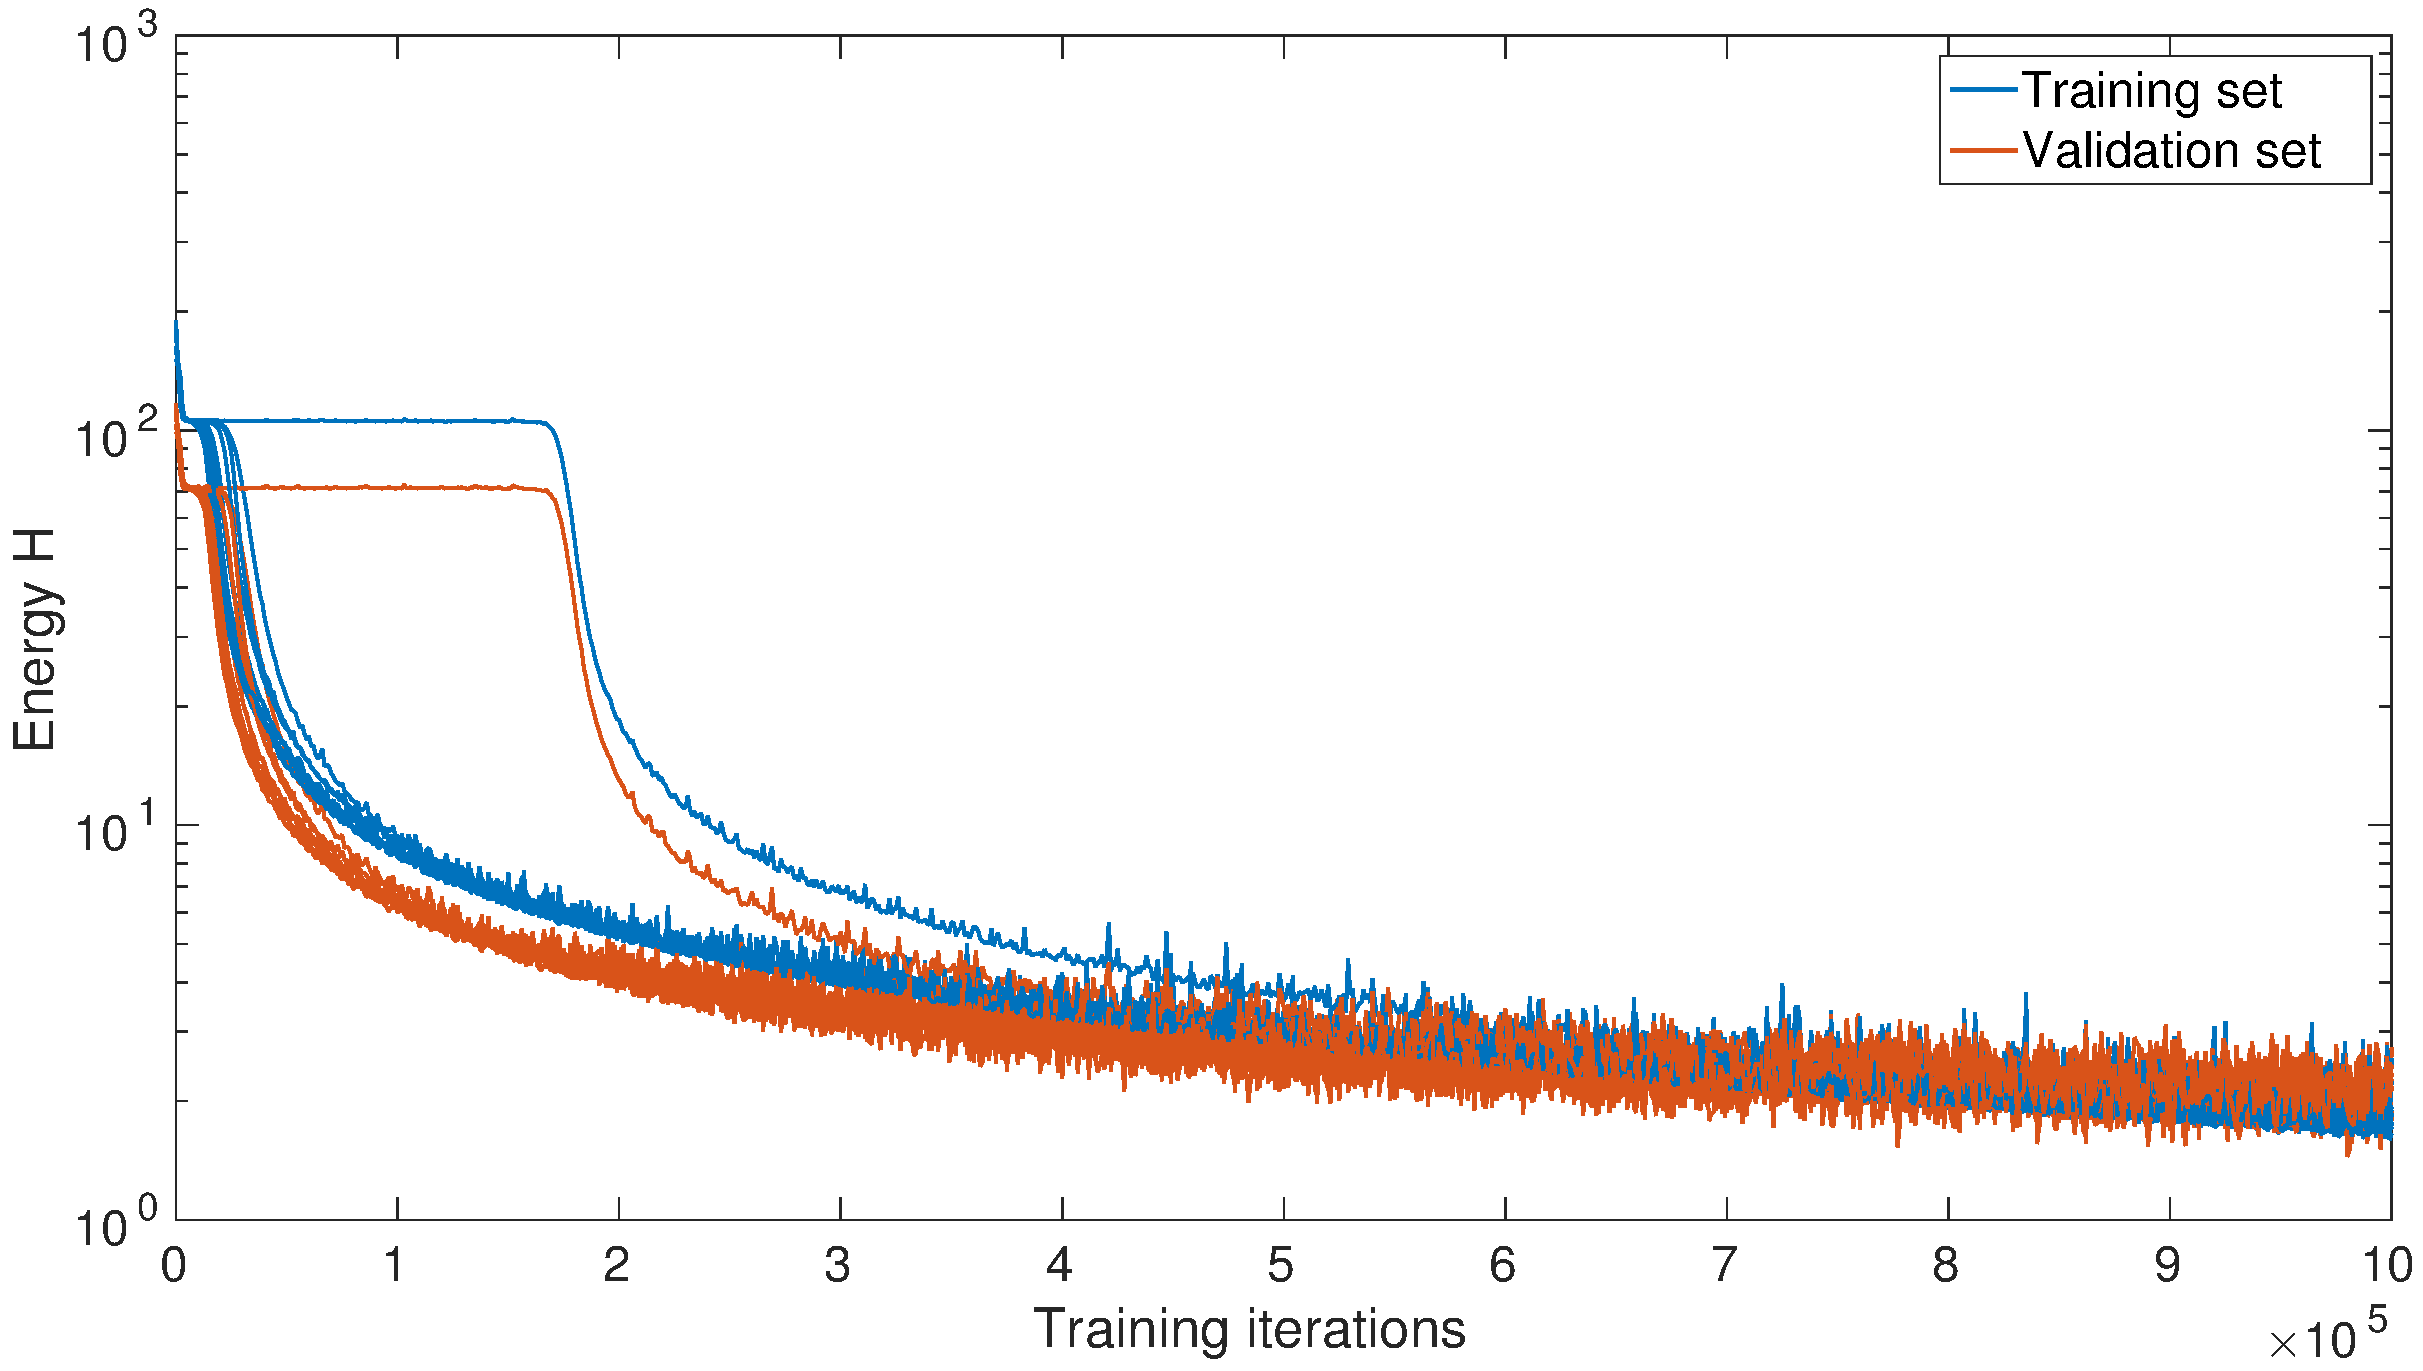
\includegraphics[width=0.7\textwidth]{../Figures/oneHL_energy.pdf}
\caption{\footnotesize Energy $H$ vs training iterations for both the training set (blue) and the validation set (red). One point every 1000 iterations is shown. Ten independently initialised runs are displayed (with the same colour-coding), y-axis is in log scale, for visual clarity.}
\label{fig:2c}
\end{figure}

\vspace*{-0.3cm}
\subsubsection*{Discussion}
\vspace*{-0.2cm}
The network architecture was then modified, by adding a hidden layer with three neurons between input and output layers. With a slight change of notation, let us denote by $\bm{V}^{(l)}$ the vector of neuron states in layer $l$, with $l = 1,\ldots,L$, and also $\bm{V}^{(0)} = \bm{\xi}^{(\mu)}$. Then, the network dynamics (proceeding forward) is governed by $\bm{V}^{(l)} = g(\bm{b}^{(l)}), \ $ where $\ \bm{b}^{(l)} = W^{(l)} \ \bm{V}^{(l-1)}\ $ and where $W^{(l)}$ is the matrix of connections between neuron layers $l-1$ and $l$.

The backpropagation training rule (proceeding backwards) can be expressed in vectorial form as ${W^{(l)} \rightarrow W^{(l)} + \delta W^{(l)}}$, with
\begin{equation}
\delta W^{(l)} =  \eta \ \bm{\delta}^{(l)} \ (\bm{V}^{(l-1)})^T \ ,\quad \text{where} \quad \bm{\delta}^{(l)} =  \begin{cases} g'(\bm{b}^{(l)}) \circ (\bm{\zeta}^{(\mu)} - \bm{V}^{(l) \mu}) \quad \ \ \text{if} \ \ l=L \\ 
g'(\bm{b}^{(l)}) \circ (W^{(l+1)})^T \bm{\delta}^{(l+1)} \quad \text{if} \ \ l < L \ .\end{cases}
\end{equation}
The symbol $\circ$ in previous equations denotes the Hadamard product (or entrywise product) between vectors of the same length. The above rules were implemented in \textsc{matlab} functions able to handle a perceptron of any size. Again, thresholds/biases were encoded inside the weight matrices $W^{(l)}$ (and thus a dummy neuron with fixed state $-1$ was added in each layer $l<L$). The program was then run with the same parameters as in part \textbf{2a}, i.e. $\eta = 0.01$, $\beta = 1/2$, ten independent runs with $10^6$ training iterations per run.

Plots in Fig.~\ref{fig:2c} show that the energy decreases, albeit non monotonically (due to the stochastic update rule), reaching very low values at the end of the training. In one case, a local minimum was found, but the algorithm was eventually able to escape from it. Performance is clearly much better than in the case of a simple perceptron, since the hidden layer allows a good approximation of the non linearly separable objective function producing the data.

\vspace*{-0.3cm}
\subsubsection*{Reference code}
\vspace*{-0.2cm}
See \textsc{matlab} script \verb!MultilayerPerceptronBackpropagation.m! and custom functions used in the script itself, in particular \verb!RunPerceptron.m!, \verb!Backpropagation.m! and \verb!ComputeErrorAndEnergy.m!.
\enlargethispage{\baselineskip}

\clearpage

\restoregeometry


\subsection*{Problem 2(d)}

\begin{table}[htbp]
\centering
\begin{tabular}{ccccc}
\toprule
   &  $\quad $ & \multicolumn{3}{c}{\textbf{Classification error $C_V$}}\\
\cmidrule{3-5}
\textbf{Run} & & \textbf{Training set}  &  $\quad $ & \textbf{Validation set}\\
\midrule
1 & &  $0.0028 \pm 0.0013$  & & $0.006 \pm 0.002$ \\
2 & &  $0.0024 \pm 0.0015$  & & $0.0054 \pm 0.0014$ \\
3 & &  $0.0024 \pm 0.0016$  & & $0.0052 \pm 0.0009$ \\
4 & &  $0.0027 \pm 0.0014$  & & $0.0052 \pm 0.0010$ \\
5 & &  $0.0026 \pm 0.0016$  & & $0.0052 \pm 0.0010$ \\
6 & &  $0.0030 \pm 0.0012$  & & $0.006 \pm 0.002$ \\
7 & &  $0.0026 \pm 0.0015$  & & $0.0053 \pm 0.0011$ \\
8 & &  $0.0026 \pm 0.0014$  & & $0.0053 \pm 0.0012$ \\
9 & &  $0.0025 \pm 0.0016$  & & $0.0055 \pm 0.0016$ \\
10 & &  $0.0025 \pm 0.0016$  & & $0.0054 \pm 0.0013$ \\
\bottomrule
\end{tabular}
\caption{\footnotesize Classification error for both the training and the validation set in ten independent training runs of a multilayer perceptron with 3 hidden neurons. Values are averages of the last $100$ values computed every $1000$ iterations, i.e. they refer to the last $100\,000$ iterations.}
\label{tab:2c}
\end{table}

\subsubsection*{Discussion}

With this network architecture (one hidden layer with three neurons), the perceptron performance in classifying input patterns increases dramatically compared to the simple perceptron with no hidden layer. 

As shown in Table~\ref{tab:2c}, the average classification error computed over the last $100\,000$ iterations is consistently below 0.01 for both the training and validation data sets, meaning that the perceptron correctly classifies more than $99\%$ of the input patterns.

The classification error of the validation data set was found to be slightly larger than that of the training set. This can be due to the fact that in the training only the training data set is used, and the noise in the data, albeit very low, can have a little effect on the perceptron performance on the validation set. %However, noise is low enough that we do not have to worry about overfitting, in this case.

Zero classification error for both the training and validation set can be actually obtained if one performs training runs in which $C_V$ is computed much more often than once every $1000$ training iterations. Some experimental runs with error evaluation every $50$ iterations, with the same parameters as in \textbf{2c}, showed that zero error can be obtained in almost all runs ($\sim 90\%$) after less than $2\cdot 10^5$ iterations, on average.

\vfill

\subsubsection*{Reference code}
\vspace*{-0.2cm}
See \textsc{matlab} script \verb!MultilayerPerceptronBackpropagation.m! and custom functions used in the script itself, in particular \verb!RunPerceptron.m!, \verb!Backpropagation.m! and \verb!ComputeErrorAndEnergy.m!.

\clearpage


\subsection*{Problem 2(e)}

\begin{figure}[H]
\centering
    \begin{subfigure}[b]{0.58\textwidth}
        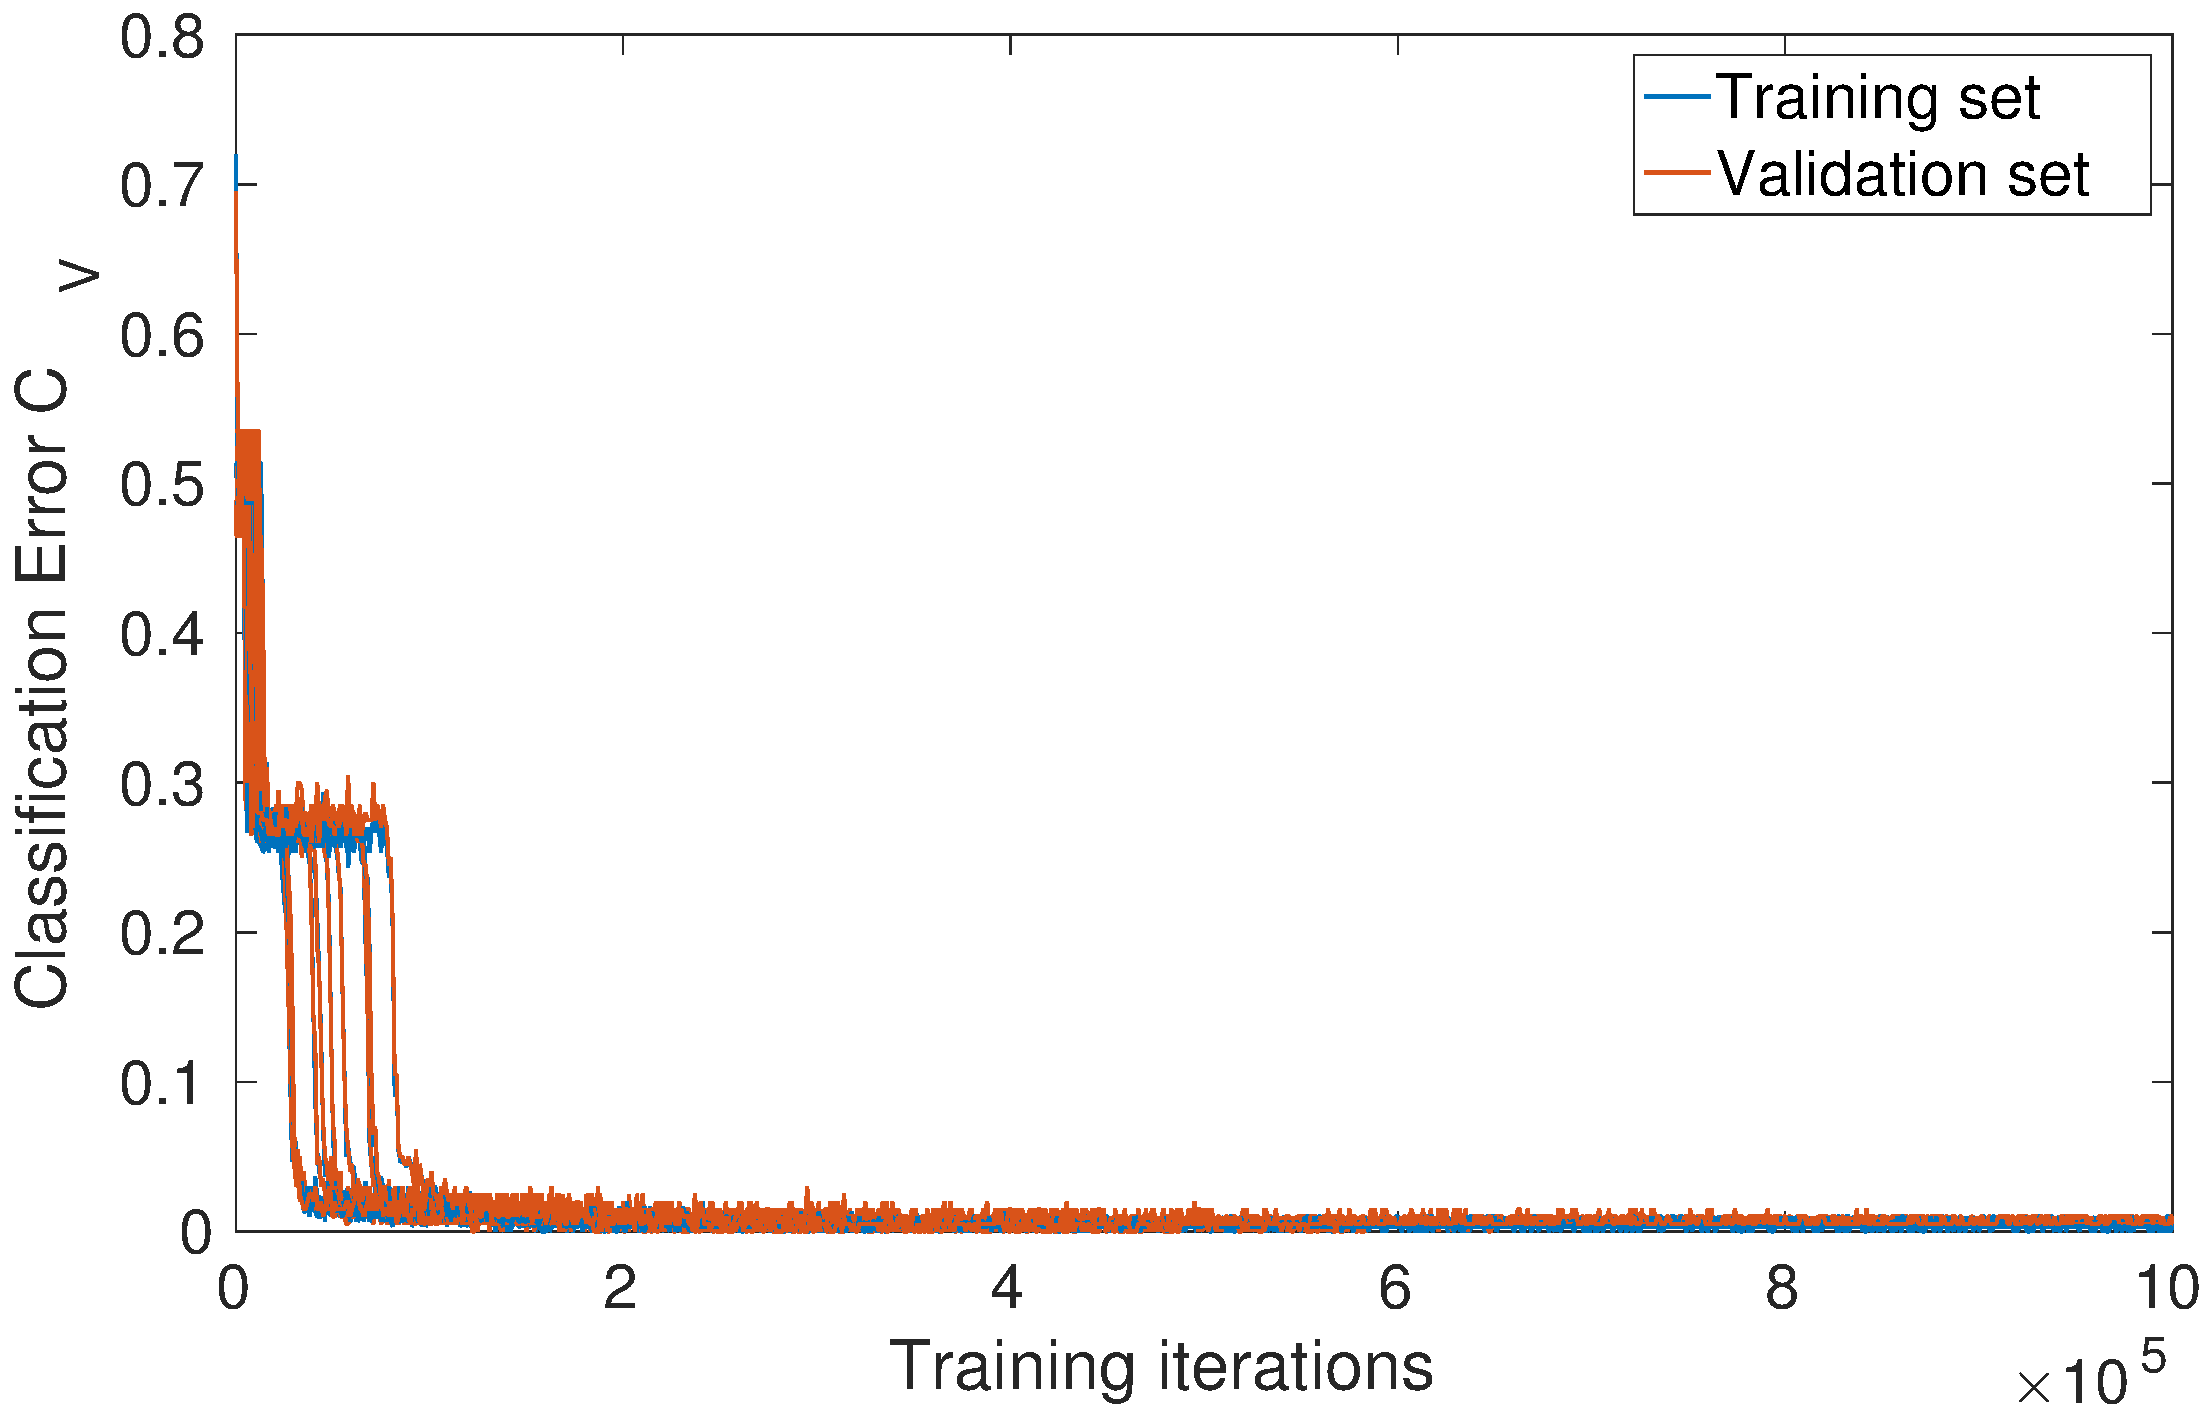
\includegraphics[width=\textwidth]{../Figures/twoHL_error.pdf}
        \caption{}
    \end{subfigure} %
    \hfill %
    \begin{subfigure}[b]{0.41\textwidth}
        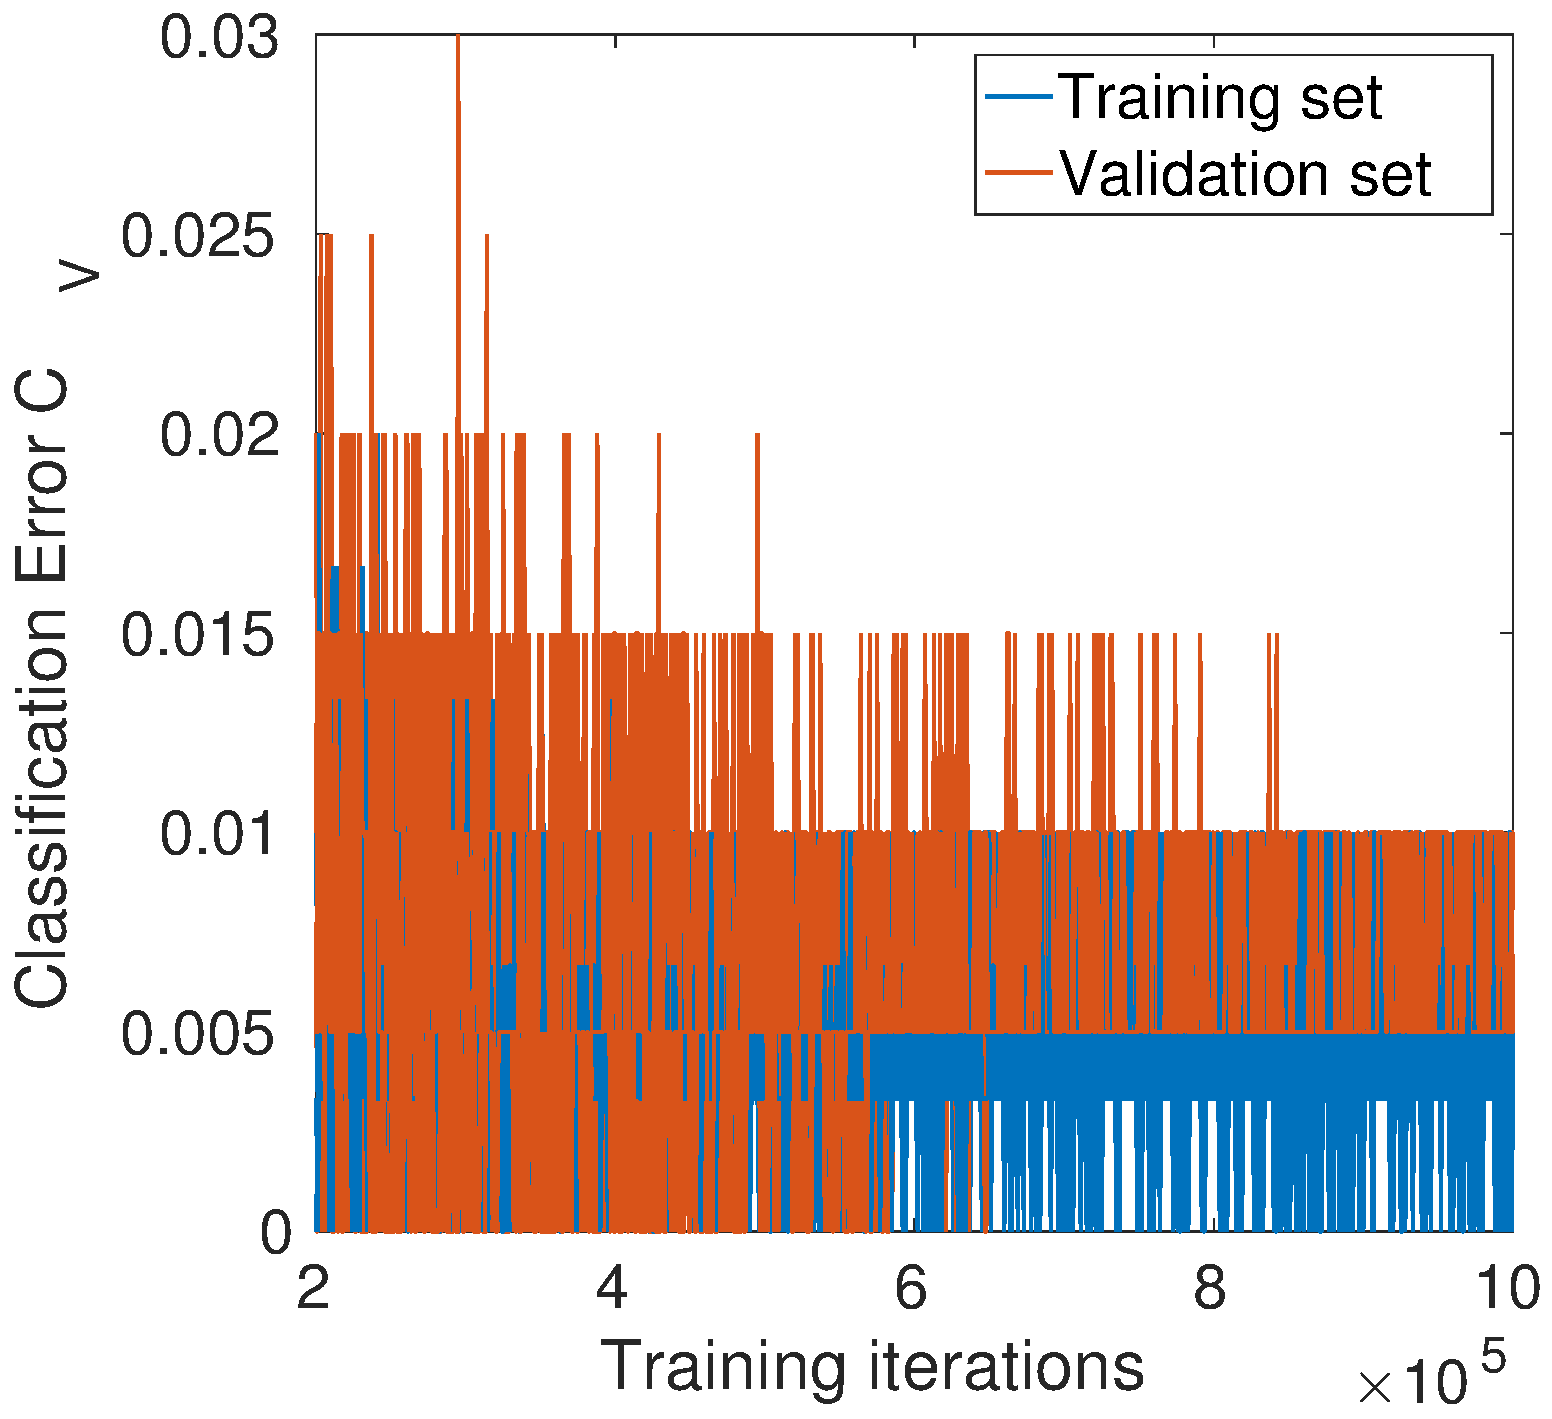
\includegraphics[width=\textwidth]{../Figures/twoHL_error_zoom.pdf}
        \caption{}
    \end{subfigure} %
\caption{\footnotesize Left panel: classification error $C_V$ vs training iterations for both the training set (blue) and the validation set (red). One point every 1000 iterations is shown. Ten independently initialised runs are displayed (with the same colour-coding). Right panel: last $800\,000$ iterations (ignoring transient phase).}
\label{fig:2e}
\end{figure}

\subsubsection*{Discussion}

The network architecture was further modified by adding a second hidden layer with two neurons. As explained in \textbf{2c}, implemented \textsc{matlab} functions \verb!RunPerceptron.m! and \verb!Backpropagation.m! can handle multilayer perceptrons of any size. 
 
Ten independent training runs were performed, with $10^6$ iterations per run and same parameters as before. The obtained classification error, computed every $1000$ iterations, is plotted in Fig~\ref{fig:2e} (left panel). Although most runs encounter local minima, in all cases the algorithm is eventually able to escape from them, reaching very small classification error. This network architecture seems therefore to give results as good as the previous one, with a single hidden layer.
 
However, consider the right panel of Fig~\ref{fig:2e}, showing a zoom-in of the left panel, without the initial transient phase. Although quite chaotic, these plots show the emergence of overfitting. In fact, after about $600\,000$ iterations, the average classification error of the validation set increases slightly and never drops below $0.005$ afterwards, whereas in the first part of the run the error frequently drops to zero (and if the training had been stopped then, zero classification error could have been achieved).

This suggests that a single hidden layer is sufficient to capture the features of the provided data sets (as can be intuitively seen by visualising the data). Adding an extra hidden layer does not significantly improve the perceptron performance as a classifier and may instead cause overfitting problems (fitting the noise in the data).

\subsubsection*{Reference code}
\vspace*{-0.2cm}
See \textsc{matlab} script \verb!MultilayerPerceptronBackpropagation.m! and custom functions used in the script itself, in particular \verb!RunPerceptron.m!, \verb!Backpropagation.m! and \verb!ComputeErrorAndEnergy.m!.

\clearpage


\appendix
\section*{Appendix: MATLAB code}

\subsection*{\texttt{MultilayerPerceptronBackpropagation.m}}

\begin{lstlisting}
%MultilayerPerceptronBackpropagation
clear
close all
tic

% =================================================================== %
% PARAMETERS
% =================================================================== %
% can specify a perceptron of L+1 layers (any L), but use 1 output neuron for safety (not tested with multiple outputs, though it should work)
networkArchitecture = [2 3 2 1]; 
beta = 0.5;
learningRate = 0.01;
weightRange = 0.2;
biasRange = 1.0;
nIterations = 1e6;
iterationsBetweenPlots = 1000;
nRuns = 10;
trainingDataPath = '../Data/train_data_new.txt';
validationDataPath = '../Data/valid_data_new.txt';
% =================================================================== %

% Read and normalize training and validation data sets
[trainingPatterns, trainingOutputs] = ReadData(trainingDataPath);
[validationPatterns, validationOutputs] = ReadData(validationDataPath);
nTraining = size(trainingPatterns,1);
nValidation = size(validationPatterns,1);
[trainingPatterns, validationPatterns] = NormalizeData(trainingPatterns, validationPatterns);

% Add dummy neuron with fixed value -1 (for including biases in weights)
trainingPatterns = [trainingPatterns, -ones(nTraining,1)];
validationPatterns = [validationPatterns, -ones(nValidation,1)];

% Initialise output data structure
x = 0:iterationsBetweenPlots:nIterations;
nPlotPoints = length(x);
emptyData = nan(1,length(x));
outputData = repmat(struct('errorTraining',emptyData,'errorValidation',emptyData,'energyTraining',emptyData,'energyValidation',emptyData),  nRuns, 1 );

%% Loop over runs
parfor run = 1:nRuns

  % Initialize random weight matrix (or, well, cell of matrices)
  weightsCell = InitialiseWeightsBiases(networkArchitecture, weightRange, biasRange);

  % Initialize plots (only use if nRuns = 1)
%     [errorHandle, trainingErrorHandle, validationErrorHandle, ...
%       energyHandle, trainingEnergyHandle, validationEnergyHandle] = InitialisePlots(x, nPlotPoints);

  tPlot = 1;

  % Compute initial classification error and energy for training set
  [trainingError, trainingEnergy] = ComputeErrorAndEnergy(weightsCell, beta, trainingPatterns, trainingOutputs);
    
  % Compute initial classification error and energy for validation set
  [validationError, validationEnergy] = ComputeErrorAndEnergy(...
    weightsCell, beta, validationPatterns, validationOutputs);
      
  % Store values
  outputData(run).errorTraining(tPlot) = trainingError;
  outputData(run).energyTraining(tPlot) = trainingEnergy;
  outputData(run).errorValidation(tPlot) = validationError;
  outputData(run).energyValidation(tPlot) = validationEnergy;
  
  for t = 1:nIterations
    
    % Pick pattern to feed (and corresponding output)
    patternID = randi(nTraining);
    inputPattern = trainingPatterns(patternID,:)';
    desiredOutput = trainingOutputs(patternID,:)';
  
    % Run perceptron
    perceptronState = RunPerceptron(inputPattern, weightsCell, beta);
  
    % Backpropagation
    weightsCell = Backpropagation(perceptronState, weightsCell, ...
      desiredOutput, beta, learningRate);

    if mod(t,iterationsBetweenPlots) == 0
      tPlot = tPlot+1;

      % Compute and store classification error and energy for training set
      [trainingError, trainingEnergy] = ComputeErrorAndEnergy(...
          weightsCell, beta, trainingPatterns, trainingOutputs);
    
      % Compute and store classification error and energy for validation set
      [validationError, validationEnergy] = ComputeErrorAndEnergy(...
          weightsCell, beta, validationPatterns, validationOutputs);
      
      % Store values
      outputData(run).errorTraining(tPlot) = trainingError;
      outputData(run).energyTraining(tPlot) = trainingEnergy;
      outputData(run).errorValidation(tPlot) = validationError;
      outputData(run).energyValidation(tPlot) = validationEnergy;
      
      % Update plots (only use if nRuns = 1)
%       UpdatePlots(tPlot, trainingErrorHandle, trainingError, ...
%         validationErrorHandle, validationError, trainingEnergyHandle, trainingEnergy, validationEnergyHandle, validationEnergy);

%       if trainingError == 0 && validationError == 0
% %         load handel
% %         sound(y,Fs)
%         fprintf('\nRUN %i: zero classification error reached. Training stopped after %i iterations.\n.', ...
%           run, t);
%         break
%       end
    end
    
  end
  
end
[errorHandle, energyHandle] = PlotErrorEnergy(outputData,x);

toc
\end{lstlisting}


\subsection*{\texttt{ReadData.m}}

\begin{lstlisting}
function [ patterns, outputs ] = ReadData( dataFilePath )
%READDATA

fileID = fopen(dataFilePath);
data = textscan(fileID, '%f %f %f');
fclose(fileID);

patterns = [data{1}, data{2}];
outputs = data{3};

end
\end{lstlisting}

\subsection*{\texttt{NormaliseData.m}}

\begin{lstlisting}
function [normalisedTrainingPatterns, normalisedValidationPatterns] = ...
    NormaliseData(trainingPatterns, validationPatterns)
%NormaliseData

n = size(trainingPatterns,1);

tmpArray = [trainingPatterns; validationPatterns];
tmpArray(:,1) = (tmpArray(:,1) - mean(tmpArray(:,1))) ...
    ./std(tmpArray(:,1));
tmpArray(:,2) = (tmpArray(:,2) - mean(tmpArray(:,2)))...
    ./std(tmpArray(:,2));

normalizedTrainingPatterns = tmpArray(1:n,:);
normalizedValidationPatterns = tmpArray(n+1:end,:);

end
\end{lstlisting}

\subsection*{\texttt{InitialiseWeightsBiases.m}}

\begin{lstlisting}
function weightsCell = InitialiseWeightsBiases(neuronsInLayers, wR, bR)
%InitialiseWeightsBiases

% wR = weightRange = 0.2;
% bR = biasRange = 1.0;

L = size(neuronsInLayers,2)-1;
weightsCell = cell(1,L);

for l = 1:L
    N = neuronsInLayers(l);
    M = neuronsInLayers(l+1);

    W = [-wR + 2*wR.*rand(M,N), -bR + 2*bR.*rand(M,1)];
    weightsCell{l} = W;
end

end
\end{lstlisting}
\clearpage

\subsection*{\texttt{RunPerceptron.m}}

\begin{lstlisting}
function perceptronState = RunPerceptron(inputPattern, weightsCell,beta)
%RUNPERCEPTRON

L = size(weightsCell,2); % L+1 layers
perceptronState = cell(1,L+1);
perceptronState{1,1} = inputPattern;

for l = 1:L
    b = beta*weightsCell{1,l}*perceptronState{1,l};
    perceptronState{1,l+1} = [tanh(b); -1]; % dummy -1 added
end

% remove dummy neuron from output layer
perceptronState{1,L+1}(end) = [];
end
\end{lstlisting}

\subsection*{\texttt{Backpropagation.m}}

\begin{lstlisting}
function updatedWeightsCell = Backpropagation(perceptronState, ...
    weightsCell, desiredOutput, beta, learningRate)
%Backpropagation

L = length(weightsCell);
updatedWeightsCell = weightsCell;

% Update connections to output neuron(s) 
gPrime = beta*(1-perceptronState{1,end}.^2); % because g = tanh
delta = (desiredOutput - perceptronState{1,end}).*gPrime;
dW = learningRate*(delta*perceptronState{1,end-1}'); % note transpose!
updatedWeightsCell{1,end} = weightsCell{1,end} + dW;

% And now backpropagate to the rest of the network (if any)
if L > 1
    for l = L-1:-1:1
        gPrime = beta*(1-(perceptronState{1,l+1}(1:end-1)).^2);
        % this is a trick to make computation easier to write and run
        tempW = weightsCell{1,l+1}';
        tempW(end,:) = [];
        delta = (tempW*delta).*gPrime;
        dw = learningRate*(delta*perceptronState{1,l}'); % transpose!
        updatedWeightsCell{1,l} = weightsCell{1,l} + dw;
    end
end

end
\end{lstlisting}

\subsection*{\texttt{ComputeErrorAndEnergy.m}}

\begin{lstlisting}
function [classificationError, energy] = ComputeErrorAndEnergy(...
    weightsCell, beta, inputPatterns, trueOutputs)
%COMPUTEERRORANDENERGY

nPatterns = size(inputPatterns, 1);
nOutputs = size(trueOutputs, 2);

perceptronOutputs = zeros(nPatterns, nOutputs);

for mu = 1:nPatterns
  perceptronState = RunPerceptron(inputPatterns(mu,:)', weightsCell, beta);
  perceptronOutputs(mu,:) = perceptronState{1,end};
end

tmpArrayError = abs(trueOutputs - sign(perceptronOutputs));
tmpArrayEnergy = (trueOutputs - perceptronOutputs).^2;
  
classificationError = 0.5/nPatterns*sum(tmpArrayError(:));
energy = 0.5*sum(tmpArrayEnergy(:));

end
\end{lstlisting}

\subsection*{\texttt{InitialisePlots.m}}

\begin{lstlisting}
function [errorHandle, trainingErrorHandle, validationErrorHandle, ...
    energyHandle, trainingEnergyHandle, validationEnergyHandle] = ...
    InitialisePlots(x, nPlotPoints)
%INITIALISEPLOTS

errorHandle = figure;
set(gcf,'color','w');
hold on;
set(errorHandle, 'Position', [100,100,800,400]);
set(errorHandle, 'DoubleBuffer','on');
xlim([0 x(end)]);
xlabel('Training iterations');
ylabel('Classification Error C_V');
set(gca, 'FontSize', 16);
trainingErrorHandle = plot(x, nan(1,nPlotPoints), 'LineWidth',1.5);
validationErrorHandle = plot(x, nan(1,nPlotPoints), 'LineWidth',1.5);
legend([trainingErrorHandle, validationErrorHandle], 'Training set', ...
    'Validation set');
hold off;
drawnow;

energyHandle = figure;
set(gcf,'color','w');
hold on;
set(energyHandle, 'Position', [1000,100,800,400]);
set(energyHandle, 'DoubleBuffer','on');
xlim([0 x(end)]);
xlabel('Training iterations');
ylabel('Energy H');
set(gca, 'FontSize', 16);
trainingEnergyHandle = plot(x, nan(1,nPlotPoints), 'LineWidth',1.5);
validationEnergyHandle = plot(x, nan(1,nPlotPoints), 'LineWidth',1.5);
legend([trainingEnergyHandle, validationEnergyHandle], 'Training set', ...
    'Validation set');
hold off;
drawnow;

end
\end{lstlisting}

\subsection*{\texttt{UpdatePlots.m}}

\begin{lstlisting}
function [] = UpdatePlots(tPlot, trainingErrorHandle, trainingError, ...
    validationErrorHandle, validationError, trainingEnergyHandle, ...
    trainingEnergy, validationEnergyHandle, validationEnergy)
%UPDATEPLOTS

plotTrainingError = get(trainingErrorHandle,'YData');
plotTrainingError(tPlot) = trainingError;
set(trainingErrorHandle,'YData', plotTrainingError);

plotValidationError = get(validationErrorHandle,'YData');
plotValidationError(tPlot) = validationError;
set(validationErrorHandle,'YData', plotValidationError);

plotTrainingEnergy = get(trainingEnergyHandle,'YData');
plotTrainingEnergy(tPlot) = trainingEnergy;
set(trainingEnergyHandle,'YData', plotTrainingEnergy);

plotValidationEnergy = get(validationEnergyHandle,'YData');
plotValidationEnergy(tPlot) = validationEnergy;
set(validationEnergyHandle,'YData', plotValidationEnergy);

drawnow;

end
\end{lstlisting}


\end{document}